
\thoughts{A reprendre, comme toutes les intros} Pour étudier la phase géométrique d'un signal $\psi$, il nous faut projeter $\psi$ sur $\PC{n}$, et ceux, tout en gardant une trace de sa phase puisque c'est le lien entre les deux qui nous intéresse. Il nous faut donc envoyer $\psi$ dans le produit :
\[\U{1}\times \PC{n}\qquad\qquad (\text{ou }\ \C^{n-1*}/\C^*)\]
\\
Garder le lien entre cet espace et celui d'origine mène à se placer dans le cadre avec d'un \emph{variété fibrée} (ou simplement fibré). Plus précisément, comme $\U{1}$ est un groupe de lie, ce sera un \emph{fibré principal} noté $S^{2n+1}\big(\U{1},\PC{n}\big)$.
\\

Comme son nom l'indique, $S^{2n+1}\big(\U{1},\PC{n}\big)$ à une structure de variété différentielle et le lien entre les $\U{1}$ et $\PC{n}$ va se faire par le biais d'une connexion. L'on verra alors que cette connexion est intrinsèquement lié à la phase dynamique du signal, et il sera discuté de la signification de ce résultat.
\\
La phase géométrique, quand à elle, sera liée avec la métrique hermitienne associée aux l'espaces projectifs complexes.
\\
Tout cela va demander quelques prérequis que nous allons voir à présent.
\\

\begin{itemize}
	\item Pour être un peu plus précis, même si $S^{2n-1}$ veut être vu comme produit le produit $\U{1}\times \PC{n-1}$, il faut pas complètement séparer les deux parce que si la phase géométrique est hérité de $\PC{n-1}$, c'est bien dans $\U{1}$ qu'elle se manifeste.
	
	\item Il s'avère que les variétés fibrées principales sont tout à fait adéquat pour décrit se double jeu entre $S^{2n-1}$ et $\U{1}\times \PC{n-1}$ et c'est dans ce cadre que la phase géométrique sera décrite et étudiée.
	
	\item Aussi, par souci de comodité, on se placera dans $\C^{n+1}$ et l'on notera la sphère unité de ce dernier :
	\[\S{n} \defeq S^{2n+1} \cong \U{1}\times \PC{n}\]
	
	\item Tout le formalisme nécessaire sera exposé dans la \cref{sec:cadre_geodiff}, avec plus de détail technique en annexe et dans la \cref{sec:phases_dans_VFP} seront décrites les différentes phases d'un point de vue géométrique.
	
\end{itemize}



\section{Cadre d'étude}\label{sec:cadre_geodiff}

Pour proprement poser le cadre, il nous faudra trois choses :
\begin{enumerate}
	
	\item D'abord faire quelque rappel de géométrie différentielle, ne serait-ce que pour fixer les notations (\Cref{subsec:rappel2geo_diff}), avec comme exemple le cas $\PC{n}$ (\Cref{subsec:PC^n_variet}), qui sera utile plus loin. 
	
	\item Ensuite, seront définies les variétés fibrés principales, avec les outils de bases qui leurs sont associés (\Cref{subsec:def2VFP}), puis $\U{1}\times \PC{n}$ sera écrit comme telle (\Cref{subsec:SUPC_VFP}).
	
	\item Enfin, il nous faudra définir une connexion sur ces fibrés, connexion qui seront, d'abord, définie de façon générale (\Cref{subsec:def2conn}), puis explicitée et interprétée dans le cas qui nous intéresse (\Cref{subsec:conn2SUPC}).
	
\end{enumerate}

\subsection{$\bf{\PC{n}}$ vue comme variété différentielle} \label{subsec:construc_PC^n}

\subsubsection{Rappels de géométrie différentielle et notations}\label{subsec:rappel2geo_diff}

Une variété différentielle se définie comme suit :
\begin{definition}[Variété différentielle] \label{defvarietoche}
	une variété différentielle de classe $C^k$ de dimension $n$ est un espace topologique
	$\manu$ munie d'un \emph{atlas} $\big\{ (\phi_i, U_i) \big\}_{i\in I}$, c'est-à-dire un ensemble finie de pair d'ouvert $U_i\subset \manu$ et d'application $\phi_i :U_i\ \lr\ \R^n$ telle que :
	\begin{itemize}
		
		\item les $U_i$ forme un recouvrement de la variété :\qquad $\bigcup_{i\in I} U_i = \manu$
		
		\item les $\phi_i$ sont des homéomorphismes sur leur image $\phi_i(U_i)\subset\R^n$.
		
		\item si l'intersection $U_i \cap U_j$ est non vide, alors ${\phi_j \circ {\phi_i}^{-1}}_{| {\phi_i}(U_i\cap U_j)}$ est un $C^k$ difféomorphisme sur son image.
		
	\end{itemize}
	A travers $\phi_i$, à tout point $x\in U_i$ sont associées des \emph{coordonnées locales} $(x^\mu)_{1\leq \mu\leq n}$, c'est-à-dire les coefficient de $\phi_i(x)$ dans une base $(e_\mu)_{1\leq \mu\leq n}$ de $\R^n$. Ces coordonnées sont dites locales car dépendantes du choix de la pair $(U_i,\phi_i)$ et la composée ${\phi_j \circ {\phi_i}^{-1}}_{| {\phi_i}(U_i\cap U_j)}$ est vue comme un \emph{changement de coordonnées}.\\
	Dans toutes la suite, toutes les objets propre au cartes seront indexes via l'alphabet classique ($i,j,k$) et le indices associées au coordonnées locales par des lettres grecs ($\mu,\nu,\alpha$).
\end{definition}

\begin{figure}[h]
	\includegraphics[width=0.6\textwidth]{fig/placeholder}
	\caption[La première figure de tout bon livre de géométrie différentielle]{La première figure de tout bon livre de géométrie différentielle : représentation de deux cartes avec l'application de changement de coordonnées}
\end{figure}

Ensuite, les \emph{espaces tangents} de $\manu$  et son fibré tangent seront respectivement notés :
\begin{align}
	\forall x\in\manu,\ &\tg[x]{\manu}  &  \tg{\manu} &= \bigsqcup_{x\in\manu}\tg[x]{\manu}
\end{align} 
Pour le dire rapidement, les vecteurs tangents agissent comme une dérivation en cela que, pour une chemin $\gamma : \R\lr\manu$, sa différentielle au point $x=\gamma(0)$ est définie par l'application :
\begin{equation} \label{eq:def2vec_tg}
	\dot{\gamma}_{x}\  :\ \begin{aligned}
		\conti[1]{\manu}{\R}\ &\lr\qquad \R \\ 
		f\qquad &\lmt\ \frac{d}{dt} f \circ\gamma(t)\Big|_{t=0} \defeq \frac{d(f \circ \gamma)}{dt}(0)
	\end{aligned}
\end{equation}
\\
Aussi, le système de coordonnées locales en $x\in\manu$ induit une base sur $\tg[x]{\manu}$, qui sera noté  $\bt_\mu = \frac{\partial}{\partial x^\mu}$. notation qui est justifié en cela que, moralement, $\bt_\mu$ dérive toute fonction test $f\in\conti[k]{\manu}{\R}$ dans le long de la $\mu^{eme}$ coordonnée (locale) de $x$.
\\

Plus généralement, si $\manu$ et $\mathpzc{N}$ sont deux variétés différentielles et $f : \manu\lr \mathpzc{N}$ une application différentiable, sa différentielle (ou application tangent ou push forward) au point $x$ est l'application linéaire qui, en coordonnée local s'écrit :
\[f_*(v) = f_*(v^\mu \bt_\mu) = \bt_\mu\big( f^\nu \big)v^\mu \Tilde{\bt}_\nu\qquad \text{ ou encore }\qquad  (f_*)_\mu^\nu = \bt_\mu\big( f^\nu \big)\]

\begin{itemize}
	
	\item fibré tangent dual
	
	\item image réciproque (``transposé'' de la différentielle)
	
	\item métrique riemannienne
	
	\item exemple : $\S{n}$, la métrique est induite par celle sur $\C^{n+1}$ et :
	\[\langle X, Y\rangle = \delta_{\mu \nu}X^\mu Y^\nu = X_\mu Y^\mu\]

	\item pour les variétés complexes, c'est un peu différente : carte holomorphe, doublage des espaces tangents
	
	\item exemple : sur $\C^{n+1}$ :
	\[\langle X, \congu{Y}\rangle = \delta_{\mu \nu}X^\mu \congu{Y}^\nu = X_\mu \congu{Y}^\mu\]
	En particulier, la passage au dual se fait sans changement les coefficients $X_\mu = X^\mu$
	
	\item forme kahlerienne :
	\begin{equation}
		\Omega = g_{\mu \congu{\alpha}} {J^{\congu{\alpha}}}_{\congu{\nu}} dw^\mu \wedge d\congu{w}^\nu
	\end{equation}
	
	\item moralement, là où $g$ fait le passage du tangent au dual, $J$ fait le passage de tangent au conjugé
	
\end{itemize}



\subsubsection{$\bf{\PC{n}}$ comme variété différentielle} \label{subsec:PC^n_variet}

Si l'espace projectif complexe à été présenté comme le quotient $\S{n}/\U{1}$, il peut aussi être vu comme :
\[\PC{n} \cong {\C^{n+1}}^*/\C^*\]
C'est-à-dire l'ensemble des classes de ${\C^{n+1}}^* = \C^{n+1} \setminus \{0_{\C^{n+1}}\}$ par la relation d'équivalence :
\[x \sim y\ \Llr\ \exists \lambda\in\C^*\ |\ x=\lambda y\]
\\
Moralement, en isolant la norme des vecteurs, ${\C^{n+1}}^*$ peut être vu comme le produit $\R^{+_*} \times \S{n}$, et de même pour $\C^*$ avec le module :
\begin{align*}
	{\C^{n+1}}^* &\cong \R^{+_*} \times \S{n}  &  \C^* &\cong \R^{+_*} \times \U{1}
\end{align*}
\\
Ainsi, le quotient par $\C^*$ revient à regarder les vecteurs de ${\C^{n+1}}^*$ modulo leur norme, puis modulo l'action de $\U{1}$. Or, ignorer la norme des vecteurs est équivalent à ne regarder que les vecteurs normées, donc les vecteurs de $\S{n}$. De façon informelle, on pourrait alors écrire\footnote{\itshape
	Ce qui s'écrit plus justement avec le troisième théorème d'isomorphisme : \[{\C^{n+1}}^*/\C^* \cong ({\C^{n+1}}^* / \R^{+_*})/(\C^* / \R^{+_*}) \cong \S{n}/\U{1} = \PC{n}\]
} :
\begin{align*}
	{\C^{n+1}}^*/\C^* &\cong {\C^{n+1}}^*/(\R^* \times \U{1})\\
	&\cong \big( {\C^{n+1}}^*/\R^* \big) /\U{1} \\
	&\cong \S{n}  / \U{1} = \PC{n} 
\end{align*}
\skipl

L'intérêt de cette écriture et que $\C^{n+1}$ est un espace vectoriel, ce qui permet de décrire $\PC{n}$ en terme de carte, ce qui se fait comme suit.
La classe de $\PC{n}$ de représentant $z = (z^i)_{0\leq i\leq n}\in{\C^{n+1}}^*$ est noté $[z]$ et on pose, $\forall i\in\llbracket0,n\rrbracket$ :
\begin{align}
	U_i &= \Big\{[z]\in\PC{n}\ \big|\ z\in \C^{n+1},\ z^i\neq 0\Big\}  &  \phi_i\  :\quad &\begin{aligned}
		U_i\ \ &\lr\quad\ \C^{i}\times \{1\} \times\C^{n-i}\cong \C^{n} \\ [z]\ \ &\lmt\ \frac{1}{z^i}z = \big(\nicefrac{z^0}{z^i},\cdots, 1, \cdots, \nicefrac{z^n}{z^i}\big)
	\end{aligned}
\end{align}
\begin{remarque}
	Si l'ensemble d'arrivé $\phi_i(U_i)$ est équivalent à un ouvert de $\C^{n}$ (l'une des composantes est constante), il est plus commode de travailler dans $\C^{n+1}$ puisque cela évite de devoir enlever et rajouter des coefficient dans les formules de changement de carte :
	\[ \forall z\in\C^{n+1}\ |\ z^{i,j}\neq 0\quad (\ie~[z]\in U_i\cap U_j) ,\qquad \phi_i \circ {\phi_j}^{-1}(z) = \frac{z^j}{z^i}z\]
\end{remarque}
\skipl
Les $(U_i,\phi_i)$ forment un atlas sur l'espace projectif complexe, faisant de ce dernier une variété de dimension $\dim = 2n$. Les $\phi_i \circ {\phi_j}^{-1}$ étant holomorphe, $\PC{n}$ est plus précisément une variété complexe de dimension complexe
, il est utile d'écrire ses coordonnées locales sous la forme $(w^\mu, \congu{w}^\mu)_{1\leq \mu \leq n}$, où :
\[\forall w\in U_i,\ \forall \mu\neq i,\quad w^\mu = \frac{z^\mu}{z^i},\qquad  \text{ où }\quad [z] = w\]
\\

Aussi, comme le produit hermitien sur ${\C^{n+1}}^*$ est invariante par la projection sur $\PC{n}$, dans le sens où\footnote{\itshape
	En terme technique, la projection sur $\PC{n}$ est une submersion riemannienne} :
\[\forall e^{i\alpha}\in\U{1},\ \forall z_{1,2}\in\C^{n+1},\quad \langle z_1 e^{i\alpha}, z_2 e^{i\alpha} \rangle = \langle z_1 , z_2 \rangle\]
il induit une métrique hermitienne sur $\PC{n}$. Plus connue sous le nom de Fubini-Study, elle s'exprime en coordonnées locales par la formule :
\begin{equation}
	\begin{aligned}
		\forall w\in\PC{n}, \forall X,Y\in\tg[w]{{\PC{n}}^+},\qquad \langle X, Y \rangle_w = g_{\mu\congu{\nu}}(w) X^\mu \congu{Y^\nu} 
		&= \frac{(1+w^\alpha \congu{w}_\alpha)\delta_{\mu\nu} - w_\mu \congu{w}_\nu}{(1+w^\alpha \congu{w}_\alpha)^2}X^\mu \congu{Y}^\nu \\
		&= \frac{1}{1+w^\alpha \congu{w}_\alpha} X^\mu \congu{Y}_\mu - \frac{w_\mu \congu{w}_\nu}{(1+w^\alpha \congu{w}_\alpha)^2} X^\mu \congu{Y}^\nu
	\end{aligned}
\end{equation}
et la forme de Kähler associée est :
\[\Omega(w) = i\frac{(1+w^\alpha \congu{w}_\alpha)\delta_{\mu\nu} - w_\mu \congu{w}_\nu}{(1+w^\alpha \congu{w}_\alpha)^2} dw^\mu \wedge d\congu{w}^\nu\]



\subsection{$\S{n}$ comme fibré principal} \label{subsec:VFP}

\subsubsection{Définition générale}\label{subsec:def2VFP}

Pour le dire simplement, les \emph{variétés fibrés} sont des variétés qui ressemble localement à des espaces produits. 
Le ruban de Modiüs en est un exemple typique : il ne peut pas s'écrire comme le produit d'un cercle avec un segment $S^{1}\times [0,1]$ à cause de la façon dont il est construit. Mais localement, une tranche du ruban est tout à fait comparable (\ie~difféomorphe) à un tel produit (\cf~\cref{fig:ruban2modius}).
\begin{figure}[h]
	\includegraphics[width=0.6\textwidth]{fig/placeholder}
	%\begin{tikzpicture}[scale=0.8]
	%\draw[opacity=0.1] (-4.5,-4.5) grid (12.5,4.5);
	
	
%%%%     MOBIUS     %%%%

	%main points
	\coordinate (s1-) at ($(90+0-30:4) + (0,-1)$);
	\coordinate (s1+) at ($(90+0+30:4) + (0,-1)$);
	
	\coordinate (s2+) at ($(90+120-30:4) + (0,-1)$);
	\coordinate (s2-) at ($(90-120+30:4) + (0,-1)$);
	
	\coordinate (s3+) at (90+120+30:4);
	\coordinate (s3-) at (90-120-30:4);
	
	%\draw (s1-) -- (s2+) -- (s3-) -- (s1-);
	%\draw (s1+) -- (s3+) -- (s2-) -- (s1+);
	%\draw (s3+) -- (s3-);
	\colorlet{tmpb}{blue!30!};
	\colorlet{tmpr}{red!30!};
	\colorlet{tmpv}{blue!30!red!30!};
	\definecolor{tmpg}{gray}{0.75};
	
	
	% bande droite
	\draw[fill=tmpr] (s1-) .. controls  ($(s1-)+(-60:3)$) and  ($(s3+)+(0:3)$) .. 
		(s3+) -- (s3-) 
		.. controls ($(s3-)+(0:1)$) and ($(s2-)+(-60:1)$) .. 
		(s2-) -- cycle;
		
	% bande haut
	\draw[fill=tmpv] (s1-) .. controls  ($(s1-)+(120:0.5)$) and  ($(s1+)+(60:0.5)$) .. 
		(s1+) -- (s2+) 
		.. controls ($(s2+)+(60:2)$) and ($(s2-)+(120:2)$) .. 
		(s2-) -- cycle;
		
	% bande gauche
	\draw[fill=tmpb] (s1+) .. controls  ($(s1+)+(-120:3)$) and  	($(s3-)+(-180:3)$) .. 
		(s3-) -- (s3+) 
		.. controls ($(s3+)+(-180:1)$) and ($(s2+)+(-120:1)$) .. 
		(s2+) -- cycle;
		
		
	%%%%     CARTE LOCALE     %%%%
	
	% ouvert U_i
	\draw (-1,0.25) -- (-1.5,2.67) node[midway, above right]{$U_i$};
	\draw (1,0.25) -- (1.5,2.67);
	
	% carte
	\draw[fill=tmpg, shift={(6.25,-1.5)}] (0,0) -- (0, 4) node[midway, left]{$G$} -- (3.5,4) -- (3.5,0) -- cycle node[midway, below]{$\pi(U_i)$};
	
	% fleche vers la carte
	\draw[-Stealth, thick] (0,2.5) ..
	controls ($(0,2.5) + (30:2)$)  and ($(7, 2) + (180-30:2)$) .. (7, 2) node[midway, above]{$h_i$};
	
\end{tikzpicture}
	\caption[Ruban de Mobius comme variété fibrée]{Représentation du ruban de Modius en tant que fibré. Les notations sont reprise de la \cref{def:VFP}.}
	\label{fig:ruban2modius}
\end{figure}
\skipl

Il existe toutes sorte de variétés fibrées dès lors qu'elles sont munies de structure remarquable. Celles qui vont nous intéresser sont celle dites principales\footnote{\itshape
	Bien que ce ne sera pas précisé, il sera toujours sous-entendu que les différentes variétés et cartes doivent avoir les mêmes niveaux de régularités pour que le tout reste cohérent.} :
\\
\begin{definition}[Variété fibrée principale] \label{def:VFP}
	Une \emph{variété fibrée principale} (VFP), ou \emph{fibré principal} est constituée de deux variétés différentielles $P$ et $B$ telles que :
	\begin{itemize}
		\item Il existe un groupe de Lie $G$ opérant à droite (ou à gauche) sur $P$ via l'application différentiable :
		\begin{equation} \label{eq:VFP_action}
			R\ :\ \begin{aligned}P\times G\ &\lr\quad\ \ P \\ (p,g)\ \ &\lmt\ R_g(p)\defeq p\cdot g = pg
			\end{aligned}
		\end{equation}
		
		\item Il existe une surjection différentiable $\ \pi:P\lr B\ $ telle que :
		\begin{equation} \label{eq:VFP_fibres}
			\forall p\in P,\quad \pi^{-1}\big(\pi(p)\big)=pG
		\end{equation}
		
		\item $P$ est munie d'un ensemble de paire $(U_i, h_i)$ tel que les $U_i$ forment un recouvrement de $B$ et tel que les $h_i : G\times U_i\lr \pi^{-1}(U_i)\subset P$ soient des difféomorphismes vérifiant :
		\begin{align*} \label{eq:VFP_atlas}
			\forall a,b\in G,\ \forall x\in B,\qquad h_i(ab,x) = h_i(a,x) \cdot b\qquad \text{et} \qquad \pi\circ h_i(a,x) = x
		\end{align*}
	\end{itemize}
	
	\begin{adjustbox}{valign=C,raise=1cm, minipage={1.1\linewidth}}
		\begin{wrapfigure}{r}{0.35\textwidth}
			\begin{tikzcd}[column sep=large]
				G\times U_i \arrow[d, "\pr{2}" left]  \arrow[r, "h" above]  & \pi^{-1}(U_i) \subset P \arrow[ld, "\pi" below right] \\
				U_i
			\end{tikzcd}
			%\caption{Digramme sûrement osef des jeux de projections entre $P$ et les cartes locales}
			\label{diagram_commu_VFP}
		\end{wrapfigure} 
		\vspace*{-0.5cm} % This is a fudge to align the top of the theorem environment with the image
		\skipl\par 
		La variété $B$ est appelé la \emph{base} de la VFP, $G$ son \emph{groupe structural} et $pG$ la \emph{fibre de $P$ passant par} $p$ et \emph{au dessus de} $\pi(p)\in B$. Le tout est notée $P(R, G, \pi, B)$ ou plus simplement $P(G,B)$.
		
		Les fibres $pG$ sont toutes difféomorphes à $G$ et $B$ est difféomorphe à $P/G$. Le diagramme commutatif ci-contre résume la situation ($\text{pr}_i$ est la projection canonique sur la $i-$ème composante).
	\end{adjustbox}
\end{definition}
\skipl 


L'ensemble $\big\{(U_i\times G, h_i)\big\}_i$ est l'équivalent d'un atlas pour les variétés différentielles classiques mais adapter pour tenir compte de la structure fibré de $P$ et de l'action de $G$. Explicité les changements de cartes dans $P$, ce fait comme suit.
\\
D'abord, $P$ étant localement difféomorphe à un produit $G\times U_i$, on peut y tracer des graphes appelés \emph{sections locales}, comme sur la \Cref{fig:section_local} \thoughts{ci-dessous}. Formellement, une section locale au dessus  de $U_i \subset B$ est une application $\sigma : U_i \lr P$ vérifiant :
\[\pi\circ \sigma = id_{{\displaystyle |}U_i}\]
\begin{figure}[H]
	\begin{floatrow}
		\ffigbox{\caption[Représentation d'une section local]
			{Représentation d'une section local $\sigma$ au dessus de $U_i\subset B$ de dimension 2. Comme $P$ n'est pas un produit à proprement parler, $\sigma$ est représenté dans $G\times U_i$ à travers $h_i$.}
			\label{fig:section_local}}{
			%\includegraphics[width=0.45\textwidth]{fig/placeholder}
			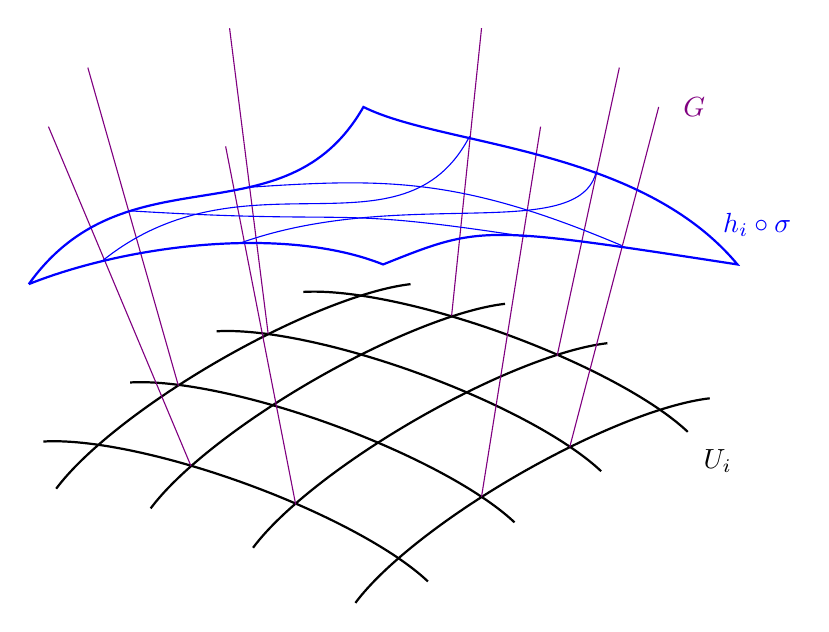
\begin{tikzpicture}%[scale=0.9]
	%\draw[opacity=0.1] (-4.5,-4.5) grid (4.5,4.5);

	%\draw (-1,-4)  .. controls (0,-2.5) and (1.5,-1.75) ..  (4,-2);

% BASE

	% gauche
	\draw[thick, xshift=1.3cm, yshift=-3.2cm, rotate=30]
		(3,0) arc [start angle=30, end angle =150, radius = 3, y radius = 0.75];
		
	\draw[thick, xshift=0cm, yshift=-2.5cm, rotate=30]
		(3,0) arc [start angle=30, end angle =150, radius = 3, y radius = 0.75];
		
	\draw[thick, xshift=-1.3cm, yshift=-2cm, rotate=30]
		(3,0) arc [start angle=30, end angle =150, radius = 3, y radius = 0.75];
		
	\draw[thick, xshift=-2.5cm, yshift=-1.75cm, rotate=30]
		(3,0) arc [start angle=30, end angle =150, radius = 3, y radius = 0.75];
		
	% droite
	\draw[thick, xshift=-2.5cm, yshift=-3cm, rotate=-20]
		(3,0) arc [start angle=30, end angle =150, radius = 3, y radius = 0.75];
	
	\draw[thick, xshift=-1.4cm, yshift=-2.25cm, rotate=-20]
		(3,0) arc [start angle=30, end angle =150, radius = 3, y radius = 0.75];
	
	\draw[thick, xshift=-0.3cm, yshift=-1.6cm, rotate=-20]
		(3,0) arc [start angle=30, end angle =150, radius = 3, y radius = 0.75];
	
	\draw[thick, xshift=0.8cm, yshift=-1.1cm, rotate=-20]
		(3,0) arc [start angle=30, end angle =150, radius = 3, y radius = 0.75];
	
	
% FIBRES

	\draw[violet] (-1.36,-3.05) -- (-2.25,1.5);
	\draw[violet] (1,-2.95) -- (1.75,1.75);
	
	\draw[violet] (-2.69,-2.56) -- (-4.5,1.75);
	\draw[violet] (2.12,-2.32) -- (3.25,2);
	
	\draw[violet] (-2.85,-1.54) -- (-4,2.5);
	\draw[violet] (1.96,-1.16) -- (2.75,2.5);
	
	\draw[violet] (-1.71,-0.88) -- (-2.2,3);
	\draw[violet] (0.62,-0.65) -- (1,3);
	
	
% SECTION

	%frame
	\draw[thick, blue] (-4.75,-0.25) .. controls (-3.5,1.5) and (-1.5,0.25) ..  
		(-0.5,2) .. controls (0.5,1.5) and (3,1.5) ..
		(4.25,0) .. controls (1,0.5) ..
		(-0.25,0) .. controls (-1.5,0.5) and (-3.5,0.25) ..
		(-4.75,-0.25);
		
	% coordo droite
	\draw[blue] (-3.45,0.68) .. controls (-0.5,0.5) and (-1,0.75) .. (1.58,0.35);
	\draw[blue] (-1.95,0.98) .. controls (-0.2,1.1) and (0.75,1.1) .. (2.78,0.24);
	
	%coordo gauche
	\draw[blue] (-3.81,0.05) .. controls (-2,1.5) and (0,0) .. (0.85,1.63);
	\draw[blue] (-2.04,0.28) .. controls (0,1) and (2.25,0.25) .. (2.46,1.19);
	
% NOTATION
	\draw (4,-2.5) node{ $U_i$};
	\draw (3.7,2) node{\color{violet} $G$};
	\draw (4.5,0.5) node{\color{blue} $h_i \circ \sigma$};
	
\end{tikzpicture}}
		
		\ffigbox{\caption[Représentation de la section canonique]
			{Représentation de la section canonique définie par rapport à $G$ avec une seconde section  $\sigma(x) = \sigma_i(x)\cdot g(x)$. Cette fois $B$ est une variété de dimension 1. % Sont également représentés leur espaces tangents horizontaux respectifs avec la transformation permettant de passer l'un à l'autre.
		}}{
			\includegraphics[width=0.45\textwidth]{fig/placeholder}
			\label{fig:section_cano}}
	\end{floatrow}
\end{figure}
\noindent
Ensuite, les hypothèses sur $P(G,B)$ sont telles que $G$ agit transitivement et librement (ou sans point fixe) sur $P$. C'est-à-dire que, sur une même fibre, tout point peut être atteint par n'importe quel autre via l'action de $G$ (transitivité) :
\begin{align*}
	\forall x\in B,\quad \forall p,q\in P_x,\ \exists t(p,q)\in G\ |\ p = q\cdot t(p,q) 
\end{align*}
et que la seule façon de laisse les points invariants par cette même action est de passer par l'élément neutre $e$ (libre) :
\begin{align*}
	\forall (p,g)\in P\times G,\quad p = p\cdot g\ \Lr\ g=e
\end{align*}
\\
De la transitivité de $G$, découle le fait que toutes les sections locales $\sigma$ au dessus de $U_i$ peuvent s'écrire à partir d'une même section $\sigma_i$ via la formule :
\[\forall x\in B,\qquad \sigma(x) = \sigma_i(x) \cdot t\big(\sigma_i(x), \sigma(x)\big)\]
Son caractère libre, lui assure l'unicité d'un choix canonique de section $\sigma_i$ sur $U_i$. Elle est donnée par :
\[{h_i}(x,e) = \sigma_i(x)\]
Cela mène à la définition :
\begin{definition}[Fonctions de transitions]
	L'intersection de deux cartes  est noté $U_{ij} = U_i\cap U_j$ et le passage d'une section local canonique est donné par :
	\[\forall x\in U_{ij},\qquad \sigma_j(x) = \sigma_i(x) t\big(\sigma_i(x), \sigma_j(x)\big)\]
	L'élément de $G$, $t(\sigma_i, \sigma_j)$, est alors appelé \emph{fonction de transition} et sera noté $\varphi_{ij}$. Elle fait effectivement la transition entre deux cartes dans le sens où :
	\[\forall (g,x)\in G\times U_{ij},\qquad {h_i}^{-1} \circ h_j(g,x) = \big( \varphi_{ij}(x)g, x \big)\]
\end{definition}
\skipl




\subsubsection{Le fibré $\bf{\VFP}$}\label{subsec:SUPC_VFP}

Dans notre cas $\S{n}$ qui fait office d'espace totale et, quant bien même il s'écrit directement comme une produit $\U{1}\times \PC{n}$, pour tenir compte du fait que $\PC{n}$ est une variété il vaut le voir localement comment le produit $\U{1}\times U_i$.
\\
Aussi, avec la normalisation sur $\S{n}$, les coordonnées locales sur $\PC{n}$ se réécrivent, $\forall w\in U_i$ :
\begin{align*}
	w^\mu = \frac{z^\mu}{z^i} &= \frac{z^\mu}{|z^i|e^{i\arg (z^i)}} = \frac{z^{\mu}}{\sqrt{1 - \sum_{\nu \neq i} |z^\nu|^2}} e^{-i\arg(z^i)}  &  \text{car }\quad \sum \big|z^\nu\big|^2 = \|z\|^2 = 1
\end{align*}
\\
On constate bien que $w^\mu$ n'est définie qu'à un choix de $e^{-i\arg z^i}\in \U{1}$ près. À l'inverse, un représentant $z_i$ dans $\S{n}$ de $w\in U_i$ aura pour coefficient :
\begin{align*}
	\forall \mu\neq i,\quad {z_i}^\mu &= \frac{w^\mu}{\|w\|}e^{i\theta}  &  {z_i}^i &= \frac{1}{\|w\|}e^{i\theta} 
\end{align*}
La norme de $w$ étant à comprendre au sens des coordonnées locales sur $U_i$\footnote{\itshape
	C'est un abus de notation, $w$ n'a pas de norme en ce sens là puisqu'elle dépend du choix de carte $U_i$. Mais ici tout le raisonnement est purement local, donc ce n'est pas un problème
} :
\begin{align*}
	\|w\|^2 = \big\|(w^\mu)_{1\leq \mu\leq n}\big\|^2 = \frac{1}{|{z_i}^i|^2}\sum_{\nu \neq i} \big|{z_i}^\nu\big|^2 = \frac{1 - |{z_i}^i|^2}{|{z_i}^i|^2} &\Llr\ \big| {z_i}^i \big|^2 \|w\|^2 = 1 - \big|{z_i}^i\big|^2 \\
	&\Llr\ \big|{z_i}^i\big|^2 = \frac{1}{1 + \|w\|^2} \\
	&\Llr\ \big|{z_i}^i\big| = \frac{1}{\sqrt{1 + w^\nu \congu{w}_\nu}}
\end{align*}
D'où l'expression des coefficients de $z_i\in\S{n}$ :
\begin{align*}
	 \forall \mu\neq i,\quad {z_i}^\mu &= \frac{w^\mu}{\sqrt{1 + w^\nu \congu{w}_\nu}}e^{i\theta}  &  {z_i}^i &= \frac{1}{\sqrt{1 + w^\nu \congu{w}_\nu}}e^{i\theta} 
\end{align*}
\\

Tout cela permet d'écrire $\S{n}$ comme une variété fibrée principale :
\begin{proposition}
	La $(2n+1)-$sphère $\S{n}$, vu comme variété plongée dans $\C^n$ est une VFP de base $\PC{n}$ et de fibre type $\U{1}$. L'action de $\U{1}$ sur $\S{n}$ étant induite par la multiplication par un scalaire complexe et où :
	\begin{itemize}
		\item La fibration $\pi$ est la projection canonique de $\S{n}$ sur $\PC{n}$ :
		\begin{equation}
			\pi\ :\ \begin{aligned} \S{n}\ &\lr\ \PC{n} \\ z\quad\ &\lmt\ \ [z]\end{aligned}
		\end{equation}
		
		\item Les cartes locales $h_i$ s'écrivent :
		\begin{equation}
			\forall w \in U_i,\ \forall e^{i\theta}\in\U{1},\  h_i(w,e^{i\theta}) = \frac{w^\mu}{\sqrt{1 + w^\nu \congu{w}_\nu}}e^{i\theta} \in \S{n}
		\end{equation}
		
		\item Les sections canoniques $\sigma_i$ au dessus des $U_i$, elles,  sont définies par :
		\begin{equation}
			\forall w \in U_i,\ \sigma_i(w) = h_i(w, 1) = \frac{w^\mu}{\sqrt{1 + w^\nu \congu{w}_\nu}}
		\end{equation}
		
		\item Les fonctions de transitions entre deux cartes $U_i$ et $U_j$ s'écrivent :
		\begin{align}
			\varphi_{ij}(w) = e^{-i \arg (z_i^i)} e^{i \arg (z_j^j)}  &  \text{ où }&\qquad z_{ij} = \phi_{ij}(w)
		\end{align}
	\end{itemize}
\end{proposition}
\skipl




\subsection{Espaces horizontaux et connexion}\label{subsec:connexion2VFP}

Pour retrouver, dans ce cadre, une notion de fréquence instantanée il va nous falloir munir $\VFP$ d'une connexion

\subsubsection{Définition général}\label{subsec:def2conn}

Comme $P$ ressemble localement à un produit $G\times U_i$, il est utile de séparer ses espaces tangents $\tg[p]{P}$ comme une somme directe d'espaces tangents respectivement aux fibres et à la base. Conformément aux représentations précédentes (\cref{fig:ruban2modius,fig:section_cano,fig:section_local}), les premiers sont appelées espaces tangents \emph{verticaux}, les seconds \emph{horizontaux} et l'on note :
\[\forall p\in P,\qquad \tg[p]{P} = \vg[p]{P} \oplus \hg[p]{P}\]
\\
Les tangents verticaux $\vg[p]{P}$ se définissent canoniquement via $\pi$, en tant que noyau de sa différentielle :
\[\vg[p]{P} \defeq \Ker (\tg[p]{\pi}) = \big\{ v\in\tg[p]{P}\ |\ \tg[p]{\pi}(v)=0 \big\}\]
\\ 
Ce n'est en revanche pas le cas des espaces horizontaux. Il faut donc faire un choix pour les $\hg[p]{P}$ et c'est ce choix qui est appelé \emph{connexion} (elle connecte les espace tangents entre eux).
Comme pour les vercticaux, ces sous-espaces peuvent être caractérisés par une 1-forme différentiable $\conn$ sur $P$ à valeur dans $\vg[p]{P}$, auquel cas :
\[\forall p\in P,\quad \hg[p]{P} = \Ker(\conn_p)\]
\skipl

Dans le cas des VFP, une connexion doit en plus avoir de bonnes propriétés au regarde de l'action de $G$ sur $P$, aboutissant à la définition :

\begin{definition}[Connexion sur VFP] \label{def:connexion2VFP}
	Une \emph{connexion} sur une VFP $P(G,B)$ est la donnée d'un sous-espace tangent, $\hg[p]{P}\subset \tg[p]{P}$, en tout point de $p\in P$ tel que :
	\begin{itemize}
		
		\item $\hg{P}$ dépend différentiellement de $p$ (``dépendre différentiellement'' à un sens précis pour les sous-espaces mais qui ne sera pas utile pour la suite).
		
		\item $\hg[p]{P}$ est supplémentaire à $\vg[p]{P}$ dans $\tg[p]{P}$ :
		\begin{equation}\label{eq:TP=V+H}
			\tg[p]{P} = \vg[p]{P} \oplus \hg[p]{P}
		\end{equation}
		
		\item l'assignation des $\hg[p]{P}$ est invariante par l'action de $G$ au sens où :
		\begin{equation}\label{eq:conn_G-inv}
			\forall (p,g)\in P\times G,\quad \hg[R_g(p)]{P} = {R_g}_* (\hg[p]{P}) = \big\{{R_g}_*(v)\ |\ v \in \hg[p]{P} \big\}
		\end{equation}
	\end{itemize}
\end{definition}
\skipl

Au delà d'assurer une compatibilité entre $H$ et $R$, l'équation \eqref{eq:conn_G-inv} permet de n'avoir à définir la connexion qu'en un seul point de chaque fibre, les autres se déduisant par cette formule. 
Concrètement, pour tout point de la base $x\in U_i$, il suffit de la définir en $\sigma_i(x) = h_i(e, x)$, de sorte que l'espace horizontale en tout autre point $\ p=h_i(g, x) = \sigma_i(x)\cdot g$ au dessus de $x$ sera donné par :
\[\hg[p]{P} = \tg[\sigma_i(x)]{R_g} (\hg[\sigma_i(x)]{P})\]
\\
De même, la 1-forme de connexion n'a besoin d'être définie que sur un point particulier au dessus de chaque fibre. Et comme tout les espaces verticaux sont difféomorphes à l'algèbre de Lie $\mathfrak{g}\cong \tg[e]{G}$ de $G$, c'est sur $\mathfrak{g}$ qu'elle est définie :

\begin{definition}[1-forme de connexion] \label{def:1-form2conn}
	La \emph{1-forme de connexion} $\conn$ d'une VFP $P(G,B)$ est définie comme la 1-forme différentiable sur $P$ à valeur dans $\mathfrak{g}$ (\ie~en tout point $p\in P$, $\conn_p$ est à valeur de $\tg[p]{P}$ dans $\mathfrak{g}$), telle que :
	\begin{equation} \label{eq:1-form2conn}
		\forall p\in P,\quad \hg[p]{P} \defeq \Ker(\conn_p)
	\end{equation}
	\skipl
	
	En terme de coordonnée local, $\conn$ elle n'a pas besoin d'être définit sur $\ U_i\times G$, mais seulement sur $\ U_i \cong U_i \times \{e\}$. Ainsi, $\conn$ induit une 1-forme sur les cartes $U_i$ par l'image réciproque des sections canonique $\sigma_i$. Elles sont notées $\locconn_i \defeq \sigma_i^*\conn$ et sur le chevauchement $U_{ij}$, elles vérifient :
	\begin{equation}\label{eq:conn_local}
		\locconn_j = {\varphi_{ij}}^{-1} \locconn_i \varphi_{ij} + {\varphi_{ij}}^{-1} \d \varphi_{ij}
	\end{equation}
\end{definition}
\skipl
\\

\begin{itemize}
	
	\item DEF horizontal+69 lift : Par abue de language, on dira de $\Tilde{\gamma}$ que c'est le relèvement horizontale de $\gamma$ si c'est le relèvement horizontale de sa projection sur $\PC{n}$ avec la condition initiale $\Tilde{\gamma}(0) = \gamma(0)$
	
	\item EDP du relèvement $g_i$ telle que $\Tilde{\gamma}(t) = h_i\big( C_\gamma(t), g_i(t) \big)$ (besoin d'un peu d'algèbre de Lie, soit annexe soit on skip les détails)
	
	\item Remarque : Même si cette notion de connexion n'est pas la même que pour les connexions affines, les deux sont très liée. En particulier si $P$ est le fibré tangent d'une variété $\manu$ avec pour groupe structural $\GL_n(\R)$, alors toute connexion sur $P$ est une connexion affine sur $\manu$ .
\end{itemize}
\skipl



\subsubsection{Choix de connexion sur $\bf{\VFP}$}\label{subsec:conn2SUPC}

\begin{itemize}
	
	\item Pour choisir la connexion est mettre sur $\VFP$, il est important de comprendre son intérêt du point de vue signal.
	
	\item Comme, à chaque instant $t$, un signal $\gamma$ sur $\S{n}$ est représenté par une pair $(e^{i\alpha(t)}, w(t))\in\U{1}\times\PC{n}$ à travers les $h_i$, il parait naturelle de voir $\alpha(t)$ comme la fréquence instantanée du signal en $\gamma(t)$.
	
	\item Le problème de ce choix est qu'il dépend de la carte $U_i$ utilisé pour représenté $\gamma(t)$, ce qui n'est pas sensé être le cas de la fréquence instantanée.
	
	\item C'est là qu'intervient la connexion : Le relèvement horizontal $\Tilde{\gamma}$ d'une courbe $C_\gamma\subset\PC{n}$, par définition, n'a pas de variation verticale. Dans notre cas, cela signifie que $\Tilde{\gamma}$ n'a pas de variation dans $\U{1}$, de variation fréquentielle.
	
	\item Bonus : Le relèvement horizontal est unique modulo un choix de phase initiale, choix de phase qui se retrouve dans les bornes d'intégrations de la phase dynamique !
	
	\item Ainsi, si $C_\gamma$ est la projection d'un signal $\gamma$, le relèvement horizontale $\Tilde{\gamma}$ s'interprète comme une version de $\gamma$ dénué de toute fréquence instantanée.
	À l'inverse, à l'instant $t$, l'action $e^{i\alpha}$ permettant de passé de $\Tilde{\gamma}(t)$ à $\gamma(t)$ est vu la fréquence instantanée du signal (voir \cref{fig:freq_inst_geodiff} ci-dessous)
	
	\begin{figure}[h]
		\includegraphics[width=0.4\textwidth]{fig/placeholder}
		\caption[Interprétation géométrique de la fréquence instantanée]{Fréquence instantanée d'un signal $\gamma$ vu comme variation vertical de $\gamma$ par rapport à son relèvement vertical $\Tilde{\gamma}$ associé}
		\label{fig:phases_p-cycl}
	\end{figure}	
	
	\item Sachant cela, es discutions de première partie suggère de poser :
	\[\forall p\in\S{n},\ \forall \bf{v}\in\tg[p]{\S{n}},\quad \conn_p(\bf{v}) = i\Im m \langle p, \bf{v}\rangle\]
	\\
	Ce qui colle tout à fait avec le fait que l'algèbre de Lie de $\U{1}$ soit $i\R$ !
	
	\item Un choix qui est doublement justifié puisque c'est également la 1-forme de connexion induite par la métrique sur $\S{n}$. \thoughts{Plus de détail dans l'annexe \ref{ann:conn2submer_riemanian} ?} (BTW c'est l'équivalent pour les VFP de la connexion de Levi-Civita)
	
	\item En effet, si $\S{n}$ n'est pas une variété complexe (problème de dimensionnalité), elle a quand-même une métrique riemannienne (réelle) induite par celle sur $\C^n$ : $\Re e\langle \cdot,\cdot\rangle$.
	
	\item Dans ce cas, les espaces horizontaux de définissent comment les espaces orthogonaux aux verticaux : 
	\[\forall p\in\S{n},\quad \hg[p]{\S{n}} = {\vg[p]{\S{n}}}^\perp\]
	
	\item Ce qui mène bien à poser $w_p = i\Im m \langle p, \cdot \rangle $ 
	
	\item Etant donné un signal $\gamma$, on peut alors voir sa fréquence instantanée à l'instant $t$ comme sa déviation au relèvement horizontale de $\gamma$. Ainsi :
	\[\phased(\gamma) = \int_{0}^t t\big( \Tilde{\gamma}(s), \gamma(s) \big)ds \]

	
\end{itemize}






\section{Interprétation des trois phases dans ce cadre} \label{sec:phases_dans_VFP}

\begin{itemize}
	
	\item Rapide résumé : On décompose tout signal multivarié complexe comme la données d'une amplitude, d'une phase et d'un ``état de polarisation''. Indépendamment de l'amplitude, cela nous ramène à travailler dans la VFP $\VFP$. La connexion 
	
	\item On la munie d'une connexion tenant compte de la métrique sur $\S{n}$, ce qui nous ramène à la définir comme la fréquence instantanée.
	
	\item Reste alors a réinterpréter les trois phases dans ce cadre
	
	\item Pour cela, d'abord un cas simple, similaire au cas particulier de la première partie : $\gamma$ pseudo-cyclique
\end{itemize}

\subsection{Cas pseudo-cyclique}

\begin{itemize}
	\item DEF : pseudo-cyclique
	
	\item Dans ce cas, la projection $C_\gamma$ de $\gamma$ sur $\PC{n}$ est (proprement) cyclique
	
	\item Comme, entre autre, Bohm l'explique dans \cite{bohm_geometric_2003}, en fonction du choix de relèvement on peut isoler les différentes phases de $\gamma$. 
	
	\item En particulier, $C_\gamma$ est cyclique, $\gamma(1)$ est dans la même fibre que $\gamma(0)$ et les trois se décrivent dans une même fibre $\gamma(0)\U{1} = \gamma(1)\U{1}$ :
	
	\item Étant donné le choix de connexion, le relèvement horizontale $\Tilde{\gamma}$ de $C_\gamma$ (à partir du point initiale $\gamma(0)$) n'a pas de phase dynamique. $\phased$ est donc donnée par différence de phase entre $\gamma(1)$ et $\Tilde{\gamma}(1)$
	
	\item Pour obtenir la phase géométrique, on considère une troisième relèvement, $\eta$, de $C_\gamma$ qui cette fois est proprement cyclique. Comme il n'a, par construction, par de phase totale, sa phase géométrique est égale à sa phase dynamique au signe près.
	
	\item Or, la phase $\phased(\eta)$ est, comme pour $\gamma$ donné par la différence de jauge entre $\Tilde{\gamma}(1)$ et $\eta(1)$.
	
	\item Tout cela est résumé par la \Cref{fig:phases_p-cycl} ci-dessous :
	\begin{figure}[h]
		\includegraphics[width=0.4\textwidth]{fig/placeholder}
		\caption[Représentation des trois phases de $\gamma$ dans le cas pseudo-cyclique]{Représentation des trois phases de $\gamma$ dans le cas pseudo-cyclique.}
		\label{fig:phases_p-cycl}
	\end{figure}
	
	\item Remarque importante : le choix de relèvement cyclique $\eta$ n'est pas unique mais n'est pas important pour autant, puisque c'est la seule propriété $\eta(0)=\eta(1)$ qui permet d'avoir l'interprétation exposé juste avant. Cela traduit, par ailleurs, l'aspect invariant par transformation de jauge de $\phaseg$.
	
	\item Ce que cette représentation montre c'est que $\phaseg$ est donné par l'holonomie du trajet $\gamma$.
	
	\item DEF : holonomie
	
		
	
	\item Dans notre cas, la variété est connexe ce qui assure que $\Hol$ est un sous-groupe de Lie connexe du groupe structural, à savoir $\U{1}$. Ainsi, $\Hol = \U{1}$, ce qui montre que (au moins dans le cas cyclique) la phase géométrique peut prendre n'importe qu'elle valeur.
	
	\item Cette formulation est très jolie mais finalement que très peu instructive. On pourrait alors se demander si $\phaseg$ ne pourrait pas, comme $\phased$, s'écrire comme l'intégrale d'une 1-forme sur $\PC{n}$.
	
	\item A cela, Mukunda \& Simon explique dans \cite{mukunda_quantum_1993} que non. Moralement, l'écriture $\phaseg = \phaset - \phased$ suggère que ça ne peut pas être le cas puisque la phase totale ne peut pas s'écrire comme l'intégrale d'une 1-forme.
	
	\item Cela vient du fait que $\phaset$ est indépendant de la trajectoire de $\gamma$ sur $]0,1[$. Au mieux, elle peut être vu comme la longueur de la géodésique $\gamma_g$ sur $\S{n}$ entre les points $\gamma(0)$ et $\gamma(1)$. C'est-à-dire comme l'intégrale de la norme sur $\S{n}$ de $\dot{\gamma}_g$ le long de $\gamma_g$. Mais rien par rapport à $\gamma$
	
\end{itemize}




\subsection{La phase géométrique dans $\PC{n}$}

\begin{itemize}
	
	\item Cela étant dit, dans le cas cyclique $\phaseg$ et $\phased$ se confonde et cette propriété peut être exploitée.
	
	\item En effet,  la commutativité de $\U{1}$ fait que $\Hol$ est indépendant du relèvement $\eta(0)$ de $C_\gamma(0)$ 
	
	\item Ajouter à cela le fait que la connexion s'exprime exclusivement dans les cartes $U_i$, on se ramène à calcul un calcul de la phase géométrique exclusivement dans $\PC{n}$.
	
	\item Dans ce cas, la phase géométrique est l'intégrale sur un lacet d'une 1-forme et le théorème de Stokes peut s'appliquer :
	
	\item THEO de Stokes
	
	\item Dans notre cas : on obtient l’intégrale d'une forme symplectique sur l'aire entouré par le lacet $C_\gamma$ (je suspecte que ce soit $-i\Im m$(métrique F-S + à affiner) 
	
	\item En somme, cela se ramène à un calcul d'aire sur $\PC{n}$
	
	\item \thoughts{Un mot sur le lien avec Fisher}
	
\end{itemize}


\subsection{Retour au cas général}

\begin{itemize}
	\item Si maintenant $\gamma$ est qu'elle conque, pour retrouver les interprétation précédente, le plus simple est encore de se ramener au cas pseudo-cyclique.
	
	\item Cela demande de refermer $\gamma$ de sorte à ne pas engendré plus de phase géométrique. En somme, on veut savoir qu'elles sont les trajectoire de $\S{n}$ qui n'engendre pas de phase géométrique.
	
	\item Sachant le représentaiton par Stokes c'est plutôt simple : 
\end{itemize}




%%%% ANNEXES %%%%



\begin{annexe}

\section{Annexe}

\subsection{Connexion induite par une métrique} \label{ann:conn2submer_riemanian}

Si $P(G,B)$ une VFP munie d'une métrique riemannienne $g$. La connexion induite par $g$ sur $P$ est définie par :
\begin{equation}
	\forall p\in P,\quad \hg[p]{P} = \vg[p]{P}^\perp
\end{equation}
\\
Plus concrètement, $\vg[p]{P}$ est isomorphe à $\mathfrak{g}$ via la transformation :
\[\forall p\in P,\ \forall a\in\mathfrak{g},\quad a^*(p) = \frac{d}{dt} p\cdot \exp(t a)\Big|_{t=0} = \frac{d}{dt} p\cdot \exp(t a)\Big|_{t=0}\defeq pa\]
\\
Avec, une base $\{\mathfrak{e}_i\}_{1\leq i\leq k}$ de $\mathfrak{g}$ induit un base $\{e_i\}_{1\leq i\leq k} = \{\mathfrak{e}^*_i\}_{1\leq i\leq k}$ sur $\vg[p]{P}$. La métrique $g$ induit alors une connexion de 1-forme :
\[\conn_g(X) = \sum_i g(X, e_i) \mathfrak{e}_i = \sum_i g_{ij}X^j \mathfrak{e}_i\]
\\
et on la projection de $X$ sur $\vg{P}$ est donnée par :
\begin{align*}
	\ver X = \conn(X)^*\quad &\Llr\quad  \ver (X^ie_i) = \sum_i g_{ij}X^j e_i \\
	&\Llr\quad  (\ver X)^i = g_{ij}X^j
\end{align*}


\subsection{Algèbre et groupe de Lie} \label{ann:2Lie}

\subsubsection{Quelques généraliés}

\subsubsection{Cas particulier : $\bf{\U{1}}$}



\subsection{Variété différentielle complexe, tiré de \cite{nakahara_geometry_2003}}\label{ann:VDC}


$\manu$ sera une \emph{variété différentielle complexe} si elle satisfait les propriétés ci-dessus où $\R^n$ est remplacé par $\C^n$ et où la condition de difféomorphisme est remplacé par la condition d'holomorphisme. 
\\
Une application $f : \C^n\lr \C^n$ étant holomorphe si chacune de ses composantes vérifie l'équation de Cauchy-Riemann :
\[\forall x,y\in\R^n,\ \forall \mu,\qquad \frac{\partial f }{\partial y^\mu}(x+iy) = i \frac{\partial f }{\partial x^\mu}(x+iy)\]
\\
Les fonctions holomorphes étant automatiquement $C^\infty$, les variétés différentielles complexes sont toujours lisse, c'est-à-dire $C^\infty$. Aussi, $\manu$ est dite de dimension complexe $n$ et dimension (réel) $2n$, notés :
\begin{align}\label{eq:manuC-base_cano}
	\dim[\C](\manu) &\defeq n  &  \dim[\R] (\manu) \defeq \dim (\manu) = 2n
\end{align}
\\

Ensuite, pour le dire rapidement, la structure complexe de $\manu$ permet de séparer les espaces tangents en deux sous espaces. Pour ce faire, on commence par noter qu'en tout point $p\in\manu$ de coordonnée $z^\nu=x^\nu+iy^\nu$, l'espace tangent $\tg[p]{\manu}$, vu comme variété réelle, admet une base :
\begin{equation}
	\tg[p]{\manu} = \vec \left\{ \frac{\partial}{\partial x^1}, \cdots, \frac{\partial}{\partial x^n}, \frac{\partial}{\partial y^1}, \cdots,  \frac{\partial}{\partial y^n} \right\}
\end{equation}
\\
Plus tôt que de se basé sur les $x^\mu$ et $y^\mu$ pour séparer les $\tg[p]{\manu}$, on définit sur ces derniers un tenseur $J_p$ de type (1,1) tel que :
\begin{align}
	J_p \frac{\partial}{\partial x^\mu} &= \frac{\partial}{\partial y^\mu}  &  J_p \frac{\partial}{\partial y^\mu} &= -\frac{\partial}{\partial x^\mu}
\end{align}
\\
Ce tenseur est l'équivalent de la multiplication par $\pm i$ et le fait que $\manu$ soit complexe assure qu'il soit défini globalement, \ie~sur $\tg{\manu}$. Il est diagonaliseable dans la base :
\begin{align}\label{eq:manuC-base_holo}
	\partial_\mu = \frac{\partial}{\partial z^\mu} &\defeq \frac{1}{2}\left( \frac{\partial}{\partial x^\mu} - i\frac{\partial}{\partial y^\mu} \right)  
	&  
	\partial_{\bar{\mu}} = \frac{\partial}{\partial \overline{z}^\mu} &\defeq \frac{1}{2}\left( \frac{\partial}{\partial x^\mu} + i\frac{\partial}{\partial y^\mu} \right)
\end{align}
\\
Ainsi en fonction de la base (\eqref{eq:manuC-base_cano} ou \eqref{eq:manuC-base_holo}), $J_p$ va s'écrire :
\begin{align}
	J_p &= \begin{pmatrix}
		\text{\large\ 0\ }\Big. & I_n \\ -I_n & \text{\large\ 0\ }\Big.
	\end{pmatrix}  &
	J_p &= \begin{pmatrix}
		iI_n & \text{\large\ 0\ }\Big. \\ \text{\large\ 0\ }\Big. & -iI_n
	\end{pmatrix} 
\end{align}
\\
Finalement, $\tg{\manu}$ peut être séparé en deux sous-espaces engendré respectivement par les $\partial_\mu$ et $\partial_{\bar{\nu}}$. On parle de vecteur holomorphe et anti-holomorphe et on note :
\begin{align}
	\tg[p]{\manu}^+ &= \Vec\big\{ \partial_\mu\ |\ 1\leq \mu\leq n \big\}  &  \tg[p]{\manu}^- &= \Vec\big\{ \partial_{\bar{\mu}}\ |\ 1\leq \mu\leq n \big\}
\end{align}

\end{annexe}


